\documentclass[a4paper,10pt]{article}
\usepackage{wasysym}
\usepackage{enumitem}
\usepackage{forloop}
\usepackage{graphicx}
\usepackage{float}
\usepackage{natbib}
\usepackage{catchfile}

% 	\newwrite\appendwrite
% \newcommand{\appendtofile}[2]{%
%     \begingroup
%     \IfFileExists{#1}%
%       {\CatchFileDef{\filecontent}{#1}{\endlinechar=`^^J\catcode\endlinechar=12\relax}}% keep existing end-of-lines
%       {\let\filecontent\empty}%
%     \immediate\openout\appendwrite=#1\relax
%     \immediate\write\appendwrite{\filecontent #2}%
%     \immediate\closeout\appendwrite
%     \endgroup
% }

\newcommand{\freq}[1]{
	% \appendtofile{\jobname_freq}{F\arabic{fReqNum}: #1}}
    [\textit{F\arabic{fReqNum}: #1}]%
    \addtocounter{fReqNum}{10}%
}

\newcommand{\freqman}[2]{
    [\textit{F#1: #2}]
}

\newcommand{\nreq}[1]{
    [\textit{N\arabic{nReqNum}: #1}]%
    \addtocounter{nReqNum}{10}%
}

\newcommand{\clar}[1]{
    [\textit{C\arabic{clarNum}: #1}]%
    \addtocounter{clarNum}{10}%
}

\newcommand{\assump}[1]{
    [\textit{A\arabic{assumpNum}: #1}]%
    \addtocounter{assumpNum}{10}%
}

\newcommand{\Qq}[1]{#1}

\newcommand{\QO}{$\Box$}% or: $\ocircle$

\newcounter{qr}
\newcommand{\Qrating}[1]{\QO\forloop{qr}{1}{\value{qr} < #1}{---\QO}}

\newcommand{\Qline}[1]{\noindent\rule{#1}{0.6pt}}

\newcounter{ql}
\newcommand{\Qlines}[1]{\forloop{ql}{0}{\value{ql}<#1}{\vskip0em\Qline{\linewidth}}}

\newenvironment{Qlist}{%
\renewcommand{\labelitemi}{\QO}
\begin{itemize}[leftmargin=1.5em,topsep=-.5em]
}{
\end{itemize}
}

\newlength{\qt}
\newcommand{\Qtab}[2]{
\setlength{\qt}{\linewidth}
\addtolength{\qt}{-#1}
\hfill\parbox[t]{\qt}{\raggedright #2}
}

\newcommand{\Qitemf}[2][]{
\begin{enumerate}[topsep=2pt,leftmargin=2.8em]
\item[\textit{F\arabic{fReqNum}#1.}] #2
\addtocounter{fReqNum}{10}
\end{enumerate}
}

\newcommand{\Qitemn}[2][]{
\begin{enumerate}[topsep=2pt,leftmargin=2.8em]
\item[\textit{N\arabic{nReqNum}#1.}] #2
\addtocounter{nReqNum}{10}
\end{enumerate}
}

\newcommand{\Qitemclar}[2][]{
\begin{enumerate}[topsep=2pt,leftmargin=2.8em]
\item[\textit{C\arabic{clarNum}#1.}] #2
\addtocounter{clarNum}{10}
\end{enumerate}
}

\title{Product Specification: blender-hand-drawn-npr}

\begin{document}
\newcounter{fReqNum}
\setcounter{fReqNum}{10}
\newcounter{nReqNum}
\setcounter{nReqNum}{10}
\newcounter{clarNum}
\setcounter{clarNum}{10}
\newcounter{assumpNum}
\setcounter{assumpNum}{10}

\maketitle
\tableofcontents

\newpage
\section{Purpose}

This document defines the Functional and Non-Functional requirements of the System. 
Critical statements are given unique IDs as follows:

\begin{itemize}
\item Functional requirements are indicated with prefix \textit{F}.
\item Non-Functional requirements are indicated with prefix \textit{N}.
\item Clarifications to initial requirements are indicated with prefix \textit{C}.
\item Assumptions are indicated with prefix \textit{A}.
\end{itemize}

Functional requirements will form the basis of User Stories (Section \ref{userstories}).
The Coverage Matrix (Appendix \ref{coveragematrix}) provides a mechanism to ensure all Functional requirements are captured as User Stories.

\newpage
\section{Initial Requirements}
\subsection{Project Brief}
This project will look at augmenting 3D rendering software to produce \nreq{high-quality} \nreq{scientific} \nreq{3D} surfaces with \nreq{pseudo hand drawn} appearance. The project will focus on extending the \nreq{Blender} [blender.org] renderer to produce these graphs, most likely via \nreq{Python} scripting.

Traditional hand drawn plots (see below) are able to \nreq{reveal structure} in 3D surfaces that is often lost in modern renders. Although modern renders have accurate light transport models, they are designed for photo realism rather than to reveal the structure of surfaces. This is particularly relevant when producing figures for \nreq{reproduction}, which must be \nreq{clear} and might only be \nreq{monochrome}.

Traditional artists developed techniques to \nreq{reveal shading} and surface features. The aim of this project will be to develop a system to produce high quality images \nreq{automatically}, according to a specification provided by a user (e.g. \freq{line-only}, \freq{highlight creases}, \freq{no lighting}).

\subsection{Customer Meetings}

\subsubsection{18-June-2018: Kick-Off (Week 1)}

\begin{itemize}
\item A \nreq{blender add-on} is to be developed which will produce images of hand-drawn appearance.
\item \nreq{Animation will not be supported}, i.e. \nreq{temporal cohesion is not a concern}.
\item \nreq{3D model will be the input}.
\item \nreq{Vector SVG will be the output}.
\item Drawing style shall reveal surface details and shape, \freq{regions of high-curvature} etc.
\item \nreq{A specific drawing style shall be chosen}, although \nreq{system design shall be flexible enough to add additional styles} at a later date.
\item \nreq{No requirement to reveal surface texture}.
\item \freq{Lines shall be scaled according to distance of the camera from the object}.
\item The approach is assumed to require Python scripting to \nreq{process render layers produced by the blender rendering engine}.
\item A nice feature to have could be to \freq{mark areas of the model which must be rendered with a line/pattern} (e.g. to draw attention to specific areas of interest, or to allow non-deterministic output).
\item User interaction will be via the existing Blender GUI. \nreq{Custom Blender GUI panels shall be developed as required to support all functionality.}
\end{itemize}

\subsubsection{25-June-2018: Weekly (Week 2)}

\begin{itemize}
\item Focus is on black and white images, however it may be useful to look at \freq{limited use of colour} (2-3 colours max).
\end{itemize}


\newpage
\section{Questionnaire}
\subsection{Non-Functional Requirements}
\subsubsection{Clarification of Initial Requirements}

\Qitemclar{\Qq{Ref N10, define the term ``high-quality''.} \Qlines{4}}
\Qitemclar{\Qq{Ref N50, state the minimum Blender version number to support.} \Qlines{1}}
\Qitemclar{\Qq{Ref N100, interpretation is ``monochrome'' means strokes will be rendered in a single colour, rather than in tones of a single colour. Please clarify if otherwise.} \Qlines{2}}
\Qitemclar{\Qq{Ref N120 and N160, interpretation is the the User will configure a Blender scene with a 3D surface mesh, including creation and positioning of a camera and any required lighting. This will be the starting point for interaction with the System. Please clarify if otherwise.} \Qlines{4}}
\Qitemclar{\Qq{Ref N170, state the minimum SVG version number to support.} \Qlines{1}}
\Qitemclar{\Qq{Ref N180, development will focus on producing stroke-based illustrations in the Pen-and-Ink style, which aligns with requirements N10, N20, N30, N40, N70, N80, N90, N100, N110, F10, F20, F30 and F40. If another illustration style is thought to be better suited, please state it here.} \Qlines{2}}
\Qitemclar{\Qq{Ref N220, if there is a preference for where the GUI panels should be located within the Blender interface, please state so here.} \Qlines{2}}

\subsubsection{Additional Requirements}

\Qitemn{\Qq{Which operating systems shall be supported? Please also indicate minimum version numbers.}
\begin{Qlist}
\item Windows: \Qline{4cm}
\item Linux: \Qline{4cm}
\item MacOS: \Qline{4cm}
\item Other: \Qline{10cm}
\end{Qlist}
}
\Qitemn{Please rate the relative importance of each of the following characteristics:
\begin{itemize}
\item Functionality \Qtab{3cm}{least important \Qrating{6} most important}
\item Reliability \Qtab{3cm}{least important \Qrating{6} most important}
\item Usability \Qtab{3cm}{least important \Qrating{6} most important}
\item Efficiency \Qtab{3cm}{least important \Qrating{6} most important}
\item Maintainability \Qtab{3cm}{least important \Qrating{6} most important}
\item Portability \Qtab{3cm}{least important \Qrating{6} most important}
\end{itemize}
}
\Qitemn{\Qq{In a few sentences, state the most critical measure of success for the System, i.e. what does a successful product look like?} \Qlines{4}}
\Qitemn{\Qq{It is assumed that only a single mesh will be present in the Scene to be rendered. Please clarify if otherwise.} \Qlines{2}}
\Qitemn{\Qq{If there are other non-functional requirements not captured by the sections above, please state them here.} \Qlines{10}}

\subsection{Functional Requirements}
\subsubsection{Clarification of Initial Requirements}

\Qitemclar{\Qq{Ref F10, interpretation ``line-only'' means only the object outline/silhouette will be rendered. Please clarify if otherwise.} \Qlines{2}}
\Qitemclar{\Qq{Ref F20, interpretation is ``highlight creases'' means only edges whose neighbouring faces meet at an angle greater than a User-defined value will be rendered. Please clarify if otherwise.} \Qlines{2}}
\Qitemclar{\Qq{Ref F30, interpretation is ``no lighting'' means only geometric data (or world data such as ambient occlusion) would be used to determine the placement of feature-highlighting strokes. Please clarify if otherwise.} \Qlines{2}}
\Qitemclar{\Qq{Ref F50, should the User have the option to toggle this stroke tapering effect on and off?}  \newline \QO{} Yes \hskip0.5cm \QO{} No}
\Qitemclar{\Qq{Ref F50, should the User have the option to influence degree of stroke taper by controlling max and min stroke thickness?} \newline \QO{} Yes \hskip0.5cm \QO{} No}
\Qitemclar{\Qq{Ref F60, selection of faces or edges will either be via the existing selection tools available in the Blender wireframe view, or by ``painting'' areas using the Blender Grease Pencil. If one particular method is more desirable, or if another method is required, please state it here.} \Qlines{4}}

\subsubsection{Additional Requirements}

\Qitemf{\Qq{Should there be natural variation in generated stroke waviness/curvature?} \newline \QO{} Yes \hskip0.5cm \QO{} No}
\Qitemf{\Qq{If yes to the above, should the User have control over the global variation of waviness/curvature?} \newline \QO{} Yes \hskip0.5cm \QO{} No}
\Qitemf{\Qq{Should there be natural variation in generated stroke thickness along the length of a stroke (independent of distance from the camera)?} \newline \QO{} Yes \hskip0.5cm \QO{} No}
\Qitemf{\Qq{If yes to the above, should the User have control over the global variation of thickness?} \newline \QO{} Yes \hskip0.5cm \QO{} No}
\Qitemf{\Qq{Should the User have control over the preferred global density of generated strokes?} \newline \QO{} Yes \hskip0.5cm \QO{} No}
\Qitemf{\Qq{Should the User have control over the directionality of generated strokes? If so, how should this be controlled?} \newline \QO{} Yes \Qline{8cm} \hskip0.5cm \QO{} No}
\Qitemf{\Qq{Should the User have control over the global stroke colour?} \newline \QO{} Yes \hskip0.5cm \QO{} No}
\Qitemf{\Qq{Should the User have control over the canvas (image background) colour?} \newline \QO{} Yes \hskip0.5cm \QO{} No}
\Qitemf{\Qq{If there are other functional requirements not captured by the sections above, please state them here.} \Qlines{10}}


\newpage
\section{Assumptions}
\begin{itemize}
\item A purely \assump{image-space} based approach will be taken, i.e. no inputs are taken from Blender's object-space.
\item \assump{It is not possible to obtain image-space data directly from Blender's render passes via the Python API}.
\item As a consequence of A20, \assump{Blender must save the required input images to disk before they can be processed by the System.}
\item As a consequence of A30, we define a new requirement: \freq{The System shall automatically activate required render passes and produce the required compositor node setup for saving these images to disk.}
\item \assump{The goal of the System is to obtain the Final Rendering for use in other software packages.}
\item As a consequence of A50, we define a new requirement: \freq{The Final Rendering shall be saved to disk, and will not be presented on-screen within Blender.}
\end{itemize}


\newpage
\section{Proposed Design}

\subsection{System Overview}

Adapted from \cite{kang2006}.
\begin{figure}[H]
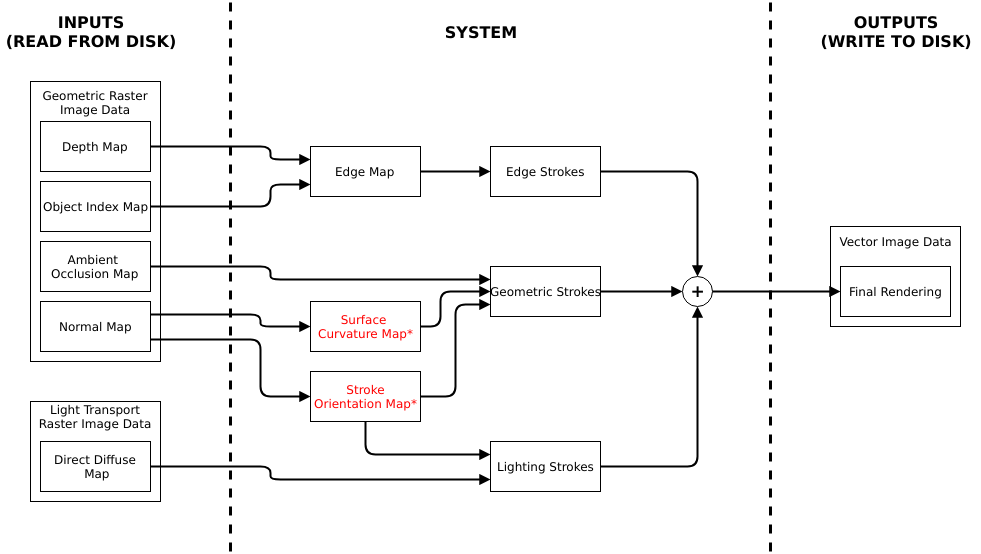
\includegraphics[width=\textwidth]{flow}
\centering
\end{figure}

\subsection{Architecture}

\begin{figure}[H]
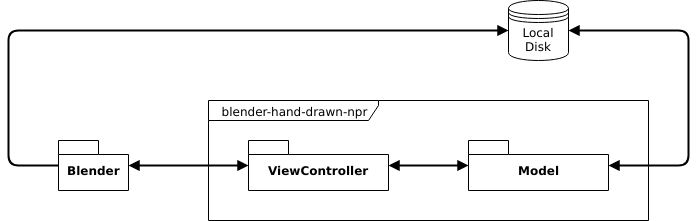
\includegraphics[width=\textwidth]{arch}
\centering
\end{figure}

\subsection{Domain Model}

Based upon \citep{hertzmann2002}, \citep{salisbury1994}, \citep{salisbury1996} and \citep{winkenbach1994}
\begin{figure}[H]
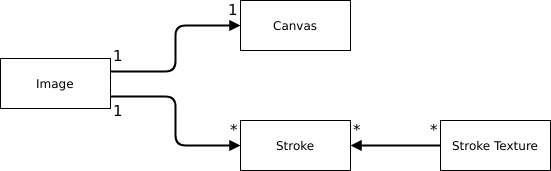
\includegraphics[width=\textwidth]{domain}
\centering
\end{figure}

\section{Risks}

To be considered upon completion of Questionnaire.

\newpage
\section{User Stories} \label{userstories}

To be considered upon completion of Questionnaire.

\appendix
\newpage
\section{Coverage Matrix} \label{coveragematrix}

To be considered upon completion of Questionnaire.
\begin{figure}[h]
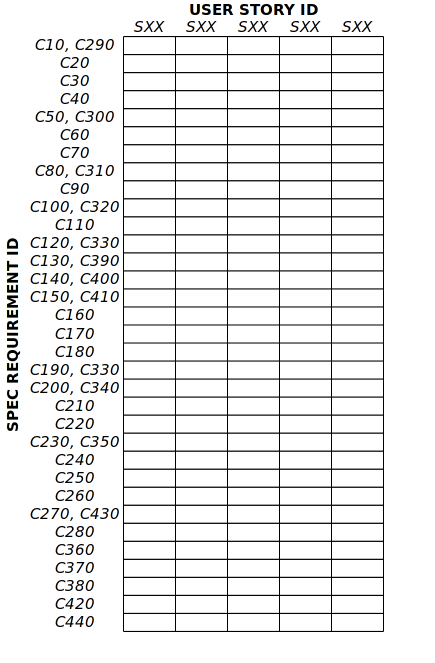
\includegraphics[width=\textwidth]{coverage_matrix}
\centering
\end{figure}

\newpage
\bibliographystyle{apalike} % Was "apa" on PC, Laptop only seems to work "apalike".
\bibliography{../dissertation/mproj}

\end{document}